%%%%%%%%%% Aquí va el código.
\subsection*{Pregunta 2.} La siguiente tabla define los tokens para un lenguaje simple donde
$\Sigma = \{a, \dotsm, z, 0, \dotsm, 9, \oplus, (, )\}$
\begin{center}
  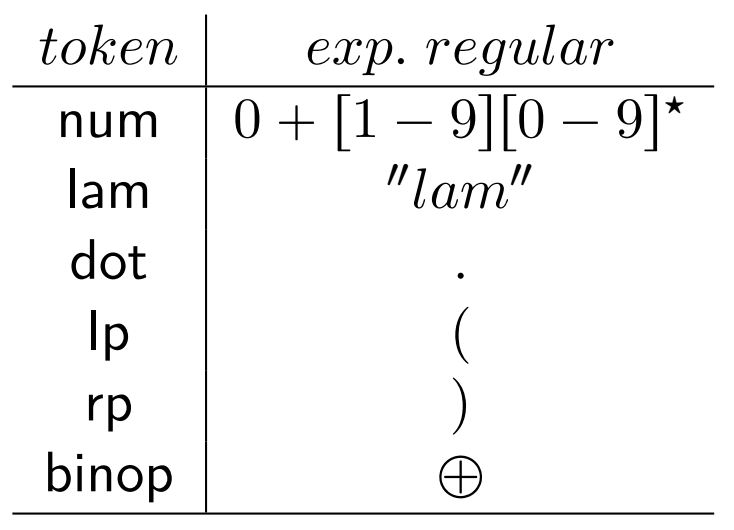
\includegraphics[scale=0.20]{./Tabla.png}
\end{center}
\begin{itemize}
\item[$a$)] Extiende la tabla anterior para agregar un token para identificadores donde la
  primera letra debe ser mayúscula seguida de cualquier secuencia de letras o números.
\item[$b$)] Construye un autómata finito determinista que acepte los tokens descritos en la tabla.
  Puedes usar algún método, eg. derivadas de expresiones regulares o construcción de un $AFN_{\epsilon}$ y
  transformaciones. Indica el método usado y muestra el proceso.
\end{itemize}

\textbf{Solución.}
\begin{itemize}
\item[$a$)] Extendiendo la tabla anterior tenemos que \newline
  \begin{center}
    \begin{tabular}{ c | c }
      \textit{token} & \textit{exp. regular} \\ \hline
      num            & $0 + [1-9][0-9]^{\star}$ \\
      lam            & ``\textit{lam}'' \\
      dot            & $\cdot$\\
      lp             & $($ \\
      rp             & $)$ \\
      binop          & $\oplus$ \\
      mi             & $[\text{A-Z}][\text{a-zA-Z}0-9]^{\star}$ \\ \hline
    \end{tabular}
  \end{center}
\item[$b$)] Para diseñar este autómata utilizaremos el método de derivaciones en expresión regular.
  Así, nuestra expresión regular sería
  \[ \text{token} = \left(\text{num } | \text{ lam } | \text{ dot } | \text{ lp } | \text{ rp } |
  \text{ binop } | \text{ mi}\right)\]
  nuestro autómata estará definido por la expresión 
  \[\text{token }\text{token}^{\star}\]
  \textbf{Obs.} No aceptamos a la cadena vacía, por tanto nuestro autómata debe tener un estado inicial
  que no sea terminal y del cuál sus transiciones a otros estados sean \underline{no} vacías. Cada estado
  final debe poder decidir si termina o regresa al inicio de nuestro autómata (pues el token en cuestión
  puede formarse de los diferentes tokens en la tabla).
  \newpage
  A continnuación se da la gráfica que represernta el autómata $AFN_{\epsilon}$ solicitado,
  este es
  \begin{center}
    \begin{tikzpicture}[estado/.style={circle,draw=black},auto,/tikz/initial text={},
        final/.style={circle,draw=black,double},thick]
      \node [estado,initial]          (i)      [left=0pt]                        {$q_1$};
      \node [estado]                  (09)     [right=20pt,     above=120pt]     {09};
      \node [estado]                  (m)      [right=20pt,     above=-90pt]     {m};
      \node [estado, final]           (num)    [right=90pt,     above=118pt]     {num};
      \node [estado, final]           (lam)    [right=148.4pt,  above=0pt]       {lam};
      \node [estado, final]           (dot)    [right=-100.8pt, above=108.8pt]   {dot};
      \node [estado, final]           (lp)     [right=-142.9pt, above=40pt]      {lp};
      \node [estado, final]           (rp)     [right=-142.9pt, above=-40pt]     {rp};
      \node [estado, final]           (binop)  [right=-100.8pt, above=-108.8pt]  {binop};
      \node [estado, final]           (mi)     [right=150pt,    above=-92pt]   {mi};
      \path[->]
      (i)     edge [curve to, out=0,in=180,relative]  node {$[1-9]$} (09)
      (09)    edge [curve to, out=0,in=180,relative]  node {$[0-9], \epsilon$} (num)
      (num)   edge [curve to, out=-25,in=155,relative]  node {$\epsilon$} (i)
      (i)   edge [curve to, out=15,in=155,relative] node {``lam''} (lam)
      (lam) edge [curve to, out=15,in=165,relative] node {$\epsilon$} (i)
      (i)     edge [curve to, out=0,in=180,relative]  node {$[\text{A-Z}]$} (m)
      (m)    edge [curve to, out=0,in=180,relative]  node {$[\text{a-zA-Z}0-9], \epsilon$} (mi)
      (mi)   edge [curve to, out=-25,in=180,relative]  node {$\epsilon$} (i)
      %
      (i)   edge [curve to, out=-15,in=155,relative] node {$\cdot$} (dot)
      (dot) edge [curve to, out=45,in=165,relative] node {$\epsilon$} (i)
      %
      (i)   edge [curve to, out=-15,in=155,relative] node {$($} (lp)
      (lp) edge [curve to, out=15,in=165,relative] node {$\epsilon$} (i)
      %
      (i)   edge [curve to, out=15,in=155,relative] node {$)$} (rp)
      (rp) edge [curve to, out=15,in=-165,relative] node {$\epsilon$} (i)
      %
      (i)   edge [curve to, out=45,in=155,relative] node {$\oplus$} (binop)
      (binop) edge [curve to, out=-15,in=-165,relative] node {$\epsilon$} (i)
      % loop's
      (num)   edge [loop right] node {$[0-9]$} (num)
      (lam)   edge [loop right] node {``lam''} (lam)
      (dot)   edge [loop left] node {$\cdot$} (dot)
      (lp)    edge [loop left] node {$($} (lp)
      (rp)    edge [loop left] node {$)$} (rp)
      (binop) edge [loop left] node {$\oplus$} (binop)
      (mi)    edge [loop right] node {$[\text{a-zA-Z}0-9]$} (mi);
    \end{tikzpicture}
  \end{center}
\end{itemize}
